\chapter{LAN Design}

\section{Hierarchical Design Model}

A hierarchical LAN design includes the following three layers, as shown in Figure \ref{Hierarchical-model}:

\begin{itemize}
\item \textbf{Access layer}  provides endpoints and users direct access to the network
\item \textbf{Distribution layer} aggregates access layers and provides connectivity to services. 
\item \textbf{Core layer} provides connectivity between distribution layers for large LAN environments.
\end{itemize}

\begin{figure}[hbtp]
\centering
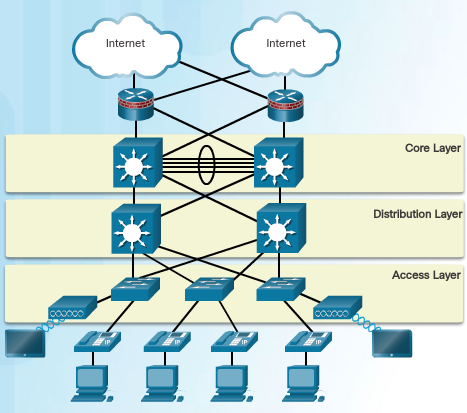
\includegraphics[width=0.7\textwidth]{pictures/Hierarchical-model.png}
\caption{Three-layer hierarchical design model}
\label{Hierarchical-model}
\end{figure}

\begin{figure}[hbtp]
\centering
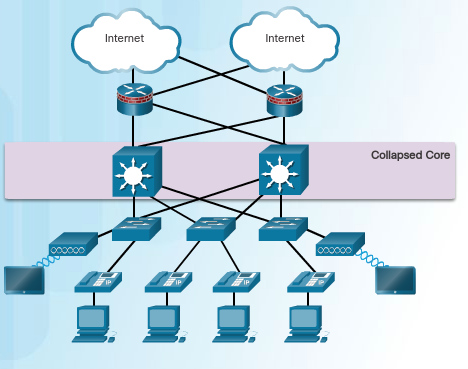
\includegraphics[width=0.7\textwidth]{pictures/collapsed-core.png}
\caption{Collapsed Core}
\label{collapsed-core}
\end{figure}

Even though the hierarchical model has three layers, some smaller enterprise networks may implement a two-tier hierarchical design. In a two-tier hierarchical design, the core and distribution layers are collapsed into one layer, as shown in Figure \ref{collapsed-core}.

\section{Expanding the network}

One method of implementing \textbf{Redundancy} is by installing duplicate equipment and providing failover services for critical devices. Another method of implementing redundancy is redundant paths.\\

A \textbf{failure domain} is the area of a network that is impacted when a critical device or network service experiences problems. The use of redundant links and reliable enterprise-class equipment minimize the chance of disruption in a network. Smaller failure domains reduce the impact of a failure on company productivity.\\

To minimize failure domain, routers or multilayer switches, are usually deployed in pairs, with access layer switches evenly divided between them. This configuration is referred to as a \textbf{switch block}. Each switch block acts independently of the others.

\paragraph{Increasing Bandwidth:} Link aggregation allows an administrator to increase the amount of bandwidth between devices by creating one logical link made up of several physical links. The EtherChannel is seen as one logical link using an EtherChannel interface. Most configuration tasks are done on the EtherChannel interface, instead of on each individual port, ensuring configuration consistency throughout the links.

\paragraph{Wireless connection:} To communicate wirelessly, end devices require a wireless NIC that incorporates a radio transmitter/receiver and the required software driver to make it operational. Additionally, a wireless router or a wireless access point (AP) is required for users to connect.

\paragraph{Fine-tuning Routing Protocols:} Advanced routing protocols, such as OSPF and EIGRP are used in large networks. Link-state routing protocols such as Open Shortest Path First (OSPF) works well for larger hierarchical networks where fast convergence is important. Another popular routing protocol for larger networks is Enhanced Interior Gateway Routing Protocol (EIGRP). Cisco developed EIGRP as a proprietary distance vector routing protocol with enhanced capabilities.

\section{Selecting network devices}

\subsection{Switch hardwares}

There are five categories of switches for enterprise networks:

\begin{itemize}
\item \textbf{Campus LAN Switches} -- To scale network performance in an enterprise LAN, there are core, distribution, access, and compact switches.
\item \textbf{Cloud-Managed Switches} -- The Cisco \textbf{Meraki} cloud-managed access switches enable virtual stacking of switches. They monitor and configure thousands of switch ports over the web, without the intervention of onsite IT staff.

\item \textbf{Data Center Switches} -- A data center should be built based on switches that promote infrastructure scalability, operational continuity, and transport flexibility. The data center switch platforms include the Cisco Nexus Series switches and the \textbf{Cisco Catalyst 6500 Series} switches.

\item \textbf{Service Provider Switches} -- Service provider switches fall under two categories: aggregation switches and Ethernet access switches. \textbf{Aggregation switches} are carrier-grade Ethernet switches that aggregate traffic at the edge of a network. \textbf{Ethernet access switches} feature application intelligence, unified services, virtualization, integrated security, and simplified management.

\item \textbf{Virtual Networking} -- Cisco \textbf{Nexus} virtual networking switch platforms provide secure multi-tenant services by adding virtualization intelligence technology to the data center network.
\end{itemize}

There are some terminologies that an administrator to be able to choose the right switch platform:

\begin{itemize}
\item \textbf{Port density} is the number of ports available on a single switch.
\item \textbf{Forwarding rates} define the processing capabilities of a switch by rating how much data the switch can process per second.
\item \textbf{Wire speed}  is the data rate that each Ethernet port on the switch is capable of attaining. Data rates can be 100 Mb/s, 1 Gb/s, 10 Gb/s, or 100 Gb/s.
\item \textbf{PoE} (Power over Ethernet) allows the switch to deliver power to a device over the existing Ethernet cabling.  This feature can be used by IP phones and some wireless access points.
\item \textbf{Multilayer switches}, so called Layer-3 switches,  are typically deployed in the core and distribution layers of an organization's switched network
\end{itemize}

\subsubsection{Router hardware}

There are three categories of routers:
\begin{itemize}
\item \textbf{Branch Routers} -- Branch routers optimize branch services on a single platform while delivering an optimal application experience across branch and WAN infrastructures.
\item \textbf{Network Edge Routers} -- Network edge routers enable the network edge to deliver high-performance, highly secure, and reliable services that unite campus, data center, and branch networks.
\item \textbf{Service Provider Routers} -- Service provider routers differentiate the service portfolio and increase revenues by delivering end-to-end scalable solutions and subscriber-aware services.
\end{itemize}
